% !TEX encoding = UTF-8
% !TEX TS-program = pdflatex
% !TEX root = ../tesi.tex

%**************************************************************
\chapter{Prodotto}
\label{cap:prodotto}
%**************************************************************

\intro{In questo capitolo viene descritto il prodotto software, la documentazione e i test eseguiti.}\\

%**************************************************************
\section{Prodotto software}
Nel corso di questa sezione vengono descritte tutte le funzionalità implementate al momento del termine dello stage.

\subsection{Login}
Il login del prodotto finale dovrà essere gestito tramite un sistema di \gls{ssog} esterno. Nonostante ciò l'implementazione di tale sistema non era tra gli obbiettivi di stage, per la demo finale è stato ritenuto sufficiente utilizzare un \gls{mockg} dello stesso. 
\begin{figure}[h]
    \begin{center}
    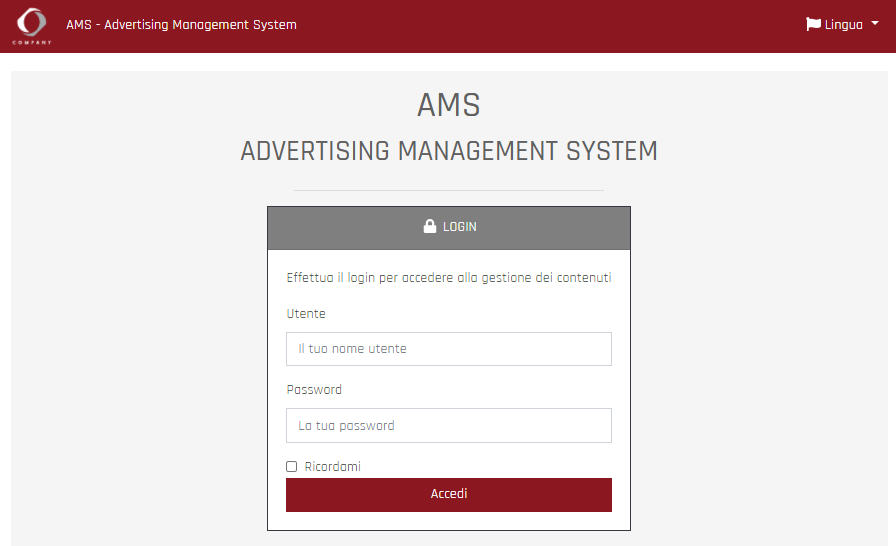
\includegraphics[width=0.95\textwidth]{login}
    \caption{Schermata di login}
    \label{fig:figure20}
    \end{center}
\end{figure}

\subsection{Scelta funzionalità}
La schermata principale del prodotto è la schermata di scelta funzionalità. Tramite questa schermata si possono raggiungere le varie funzioni offerte dal prodotto.
\begin{figure}[h]
    \begin{center}
    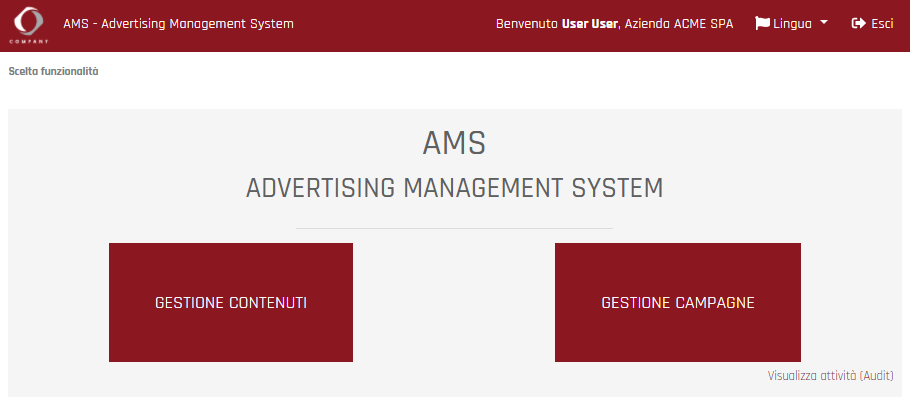
\includegraphics[width=1\textwidth]{funzionalita}
    \caption{Schermata di scelta funzionalità}
    \label{fig:figure21}
    \end{center}
\end{figure}
Più nello specifico, le funzionalità raggiungibili tramite questa schermata sono:
\begin{itemize}
    \item gestione dei contenuti;
    \item gestione delle campagne (Non abilitata);
    \item visualizzazione audit.
\end{itemize}

\subsection{Gestione contenuti}
Tramite la schermata di gestione contenuti è possibile raggiungere le sezioni di lavoro divise per ruolo (Editore, Redattore, Supervisore).
\begin{figure}[h]
    \begin{center}
    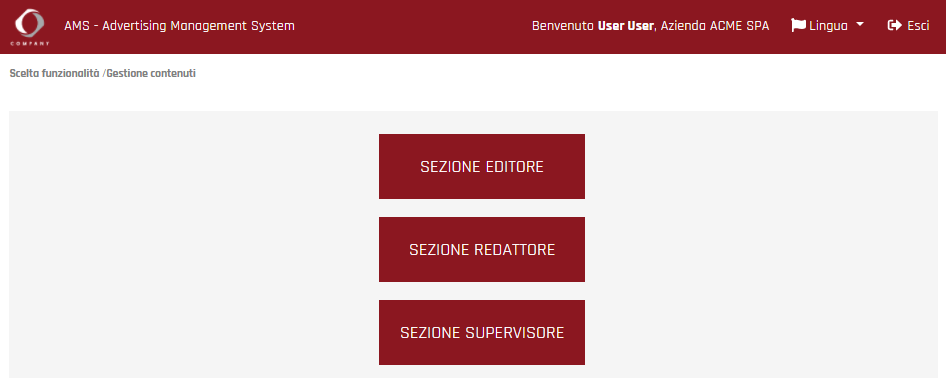
\includegraphics[width=1\textwidth]{gestcont}
    \caption{Schermata di gestione contenuti}
    \label{fig:figure22}
    \end{center}
\end{figure}
\\Ovviamente ogni utente puo visualizzare solamente le sezioni relative ai ruoli a lui assegnati.

\subsection{Sezione editore}
Questa sezione è quella in cui sono utilizzabili la maggior parte delle funzionalità obbiettivo dello stage. In questa schermata è visualizzata una lista di tutti i \gls{contenutog}. Per ciascuno di questi è possibile:
\begin{itemize}
    \item visualizzarne l'anteprima;
    \item clonarlo;
    \item modificarlo;
    \item richiederne l'associazione;
    \item eliminarlo.
\end{itemize}
Nel caso sia stata richiesta l'associazione di un contenuto, questo non potra più essere eliminato né modificato.
Tramite questa pagina è inoltre possibile creare un nuovo contenuto.
\begin{figure}[h]
    \begin{center}
    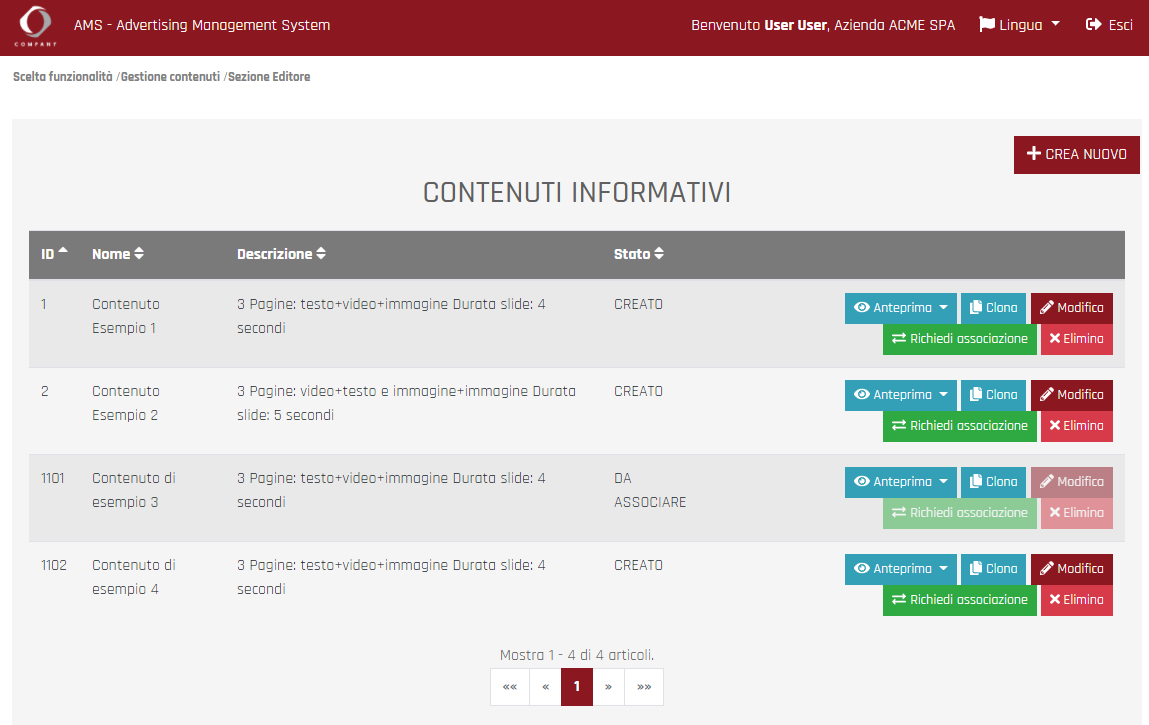
\includegraphics[width=1\textwidth]{editore}
    \caption{Schermata di gestione contenuti}
    \label{fig:figure23}
    \end{center}
\end{figure}

\subsection{Creazione di un contenuto}
La schermate di creazione di un contenuto è divisa in due aree. In quella di sinistra si inseriscono le informazioni generali relative al contenuto. In quella di destra è possibile creare le pagine del contenuto, selezionando per ciascuna uno tra i vari template disponibili.
Nel caso si scelgano template con contenuti multimediali è sufficiente che questi vengano caricati attraverso l'apposito pulsante. Nel caso ci siano contenuti testuali da inserire è possibile invece utilizzare l'apposito editor di testo.
\begin{figure}[h]
    \begin{center}
    \includegraphics[width=1\textwidth]{Creazione}
    \caption{Creazione di un contenuto}
    \label{fig:figure24}
    \end{center}
\end{figure}

\subsection{Anteprima di un contenuto}
La possibilità di visualizzare l'anteprima di un contenuto una volta creato è una delle funzionalità più utili e importanti. L'anteprima ermette infatti di visualizzare come sarebbe un contenuto una volta pubblicato e permette di decidere se richiederne l'associazione o modificarlo.
\begin{figure}[h]
    \begin{center}
    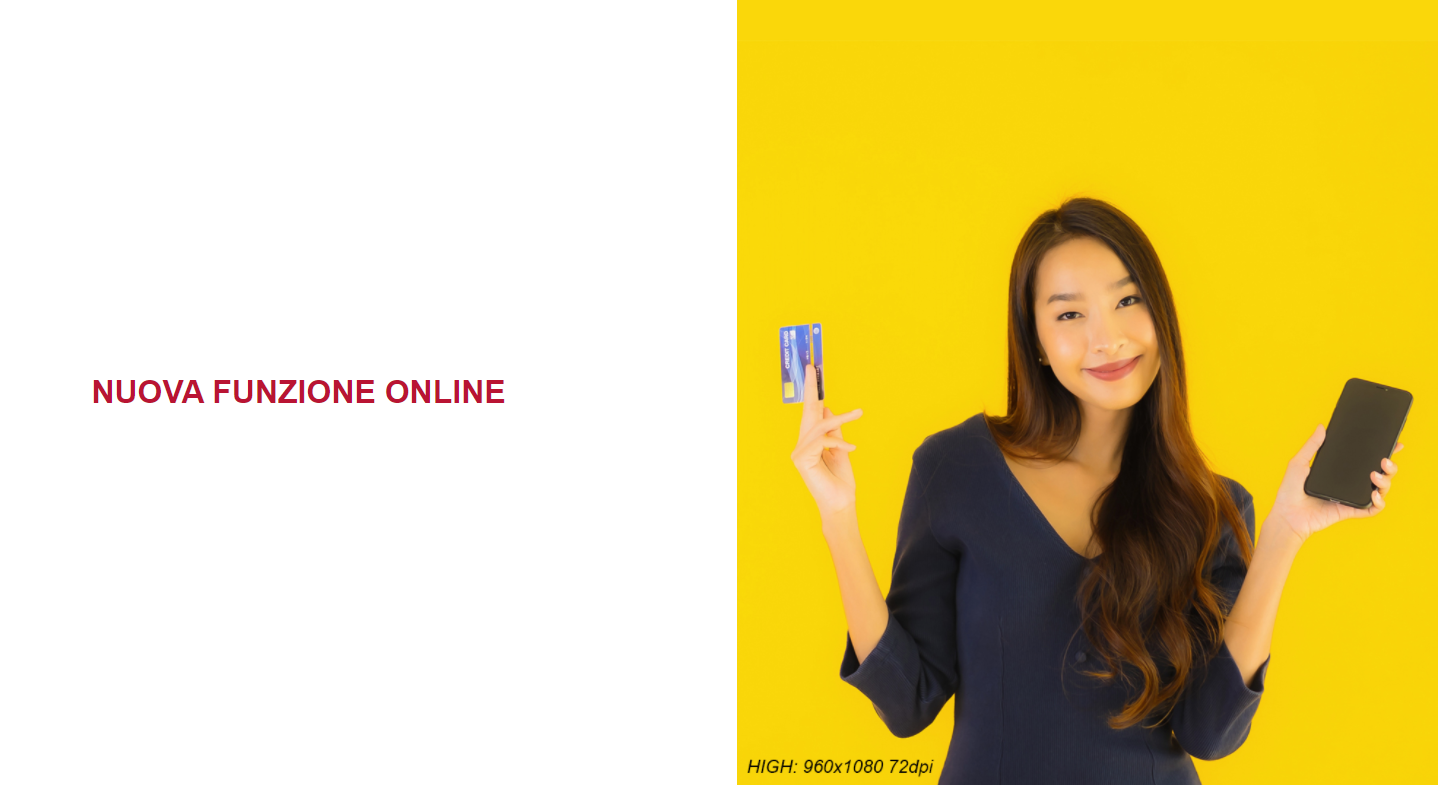
\includegraphics[width=1\textwidth]{anteprima}
    \caption{Anteprima di un contenuto di esempio}
    \label{fig:figure25}
    \end{center}
\end{figure}

\subsection{Clonazione di un contenuto}
La possibilità di clonare un contenuto è utile nel caso si voglia creare un contenuto simile ad uno già pubblicato senza la necessità di dover partire da zero. Per clonare un contenuto è sufficiente cliccare su \textit{"Clona"} nella sezione dedicata al ruolo di editore. Fatto ciò si aprirà automaticamente un pannello modale in cui è necessario inserire il nome che si vuole assegnare al nuovo contenuto.
\begin{figure}[h]
    \begin{center}
    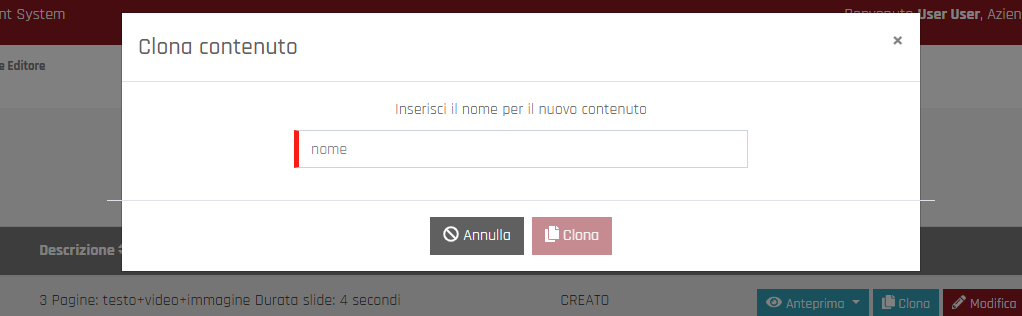
\includegraphics[width=1\textwidth]{clona}
    \caption{Clonazione di un contenuto}
    \label{fig:figure26}
    \end{center}
\end{figure}

\subsection{Modifica di un contenuto}
Modificare un contenuto può essere indispensabile nel caso, ad esempio, siano state inserite immagini o testi errati. La schermata di modifica di un contenuto si presenta in modo analogo a quella di creazione con la differenza che i campi dati hanno già le informazioni del contenuto al loro interno.
\begin{figure}[h]
    \begin{center}
    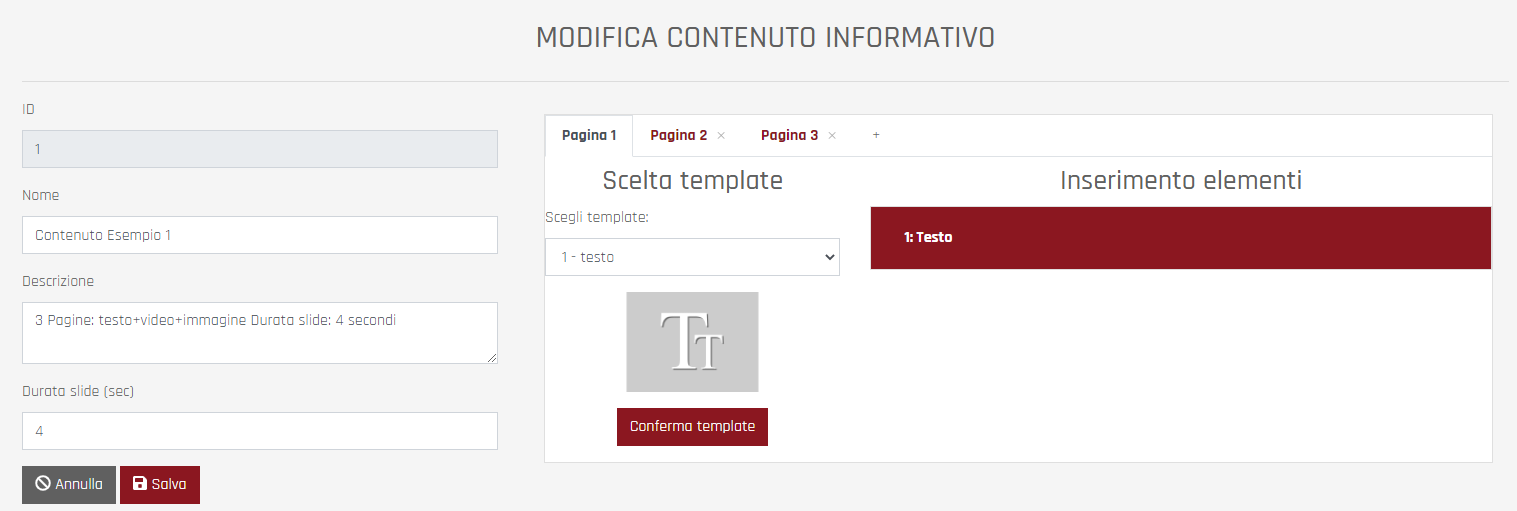
\includegraphics[width=1\textwidth]{modifica}
    \caption{Modifica di un contenuto}
    \label{fig:figure27}
    \end{center}
\end{figure}
\newpage
\subsection{Associazione di un contenuto}
La richiesta di associazione di un contenuto è il primo passo da eseguire perchè questo possa essere pubblicato. Una volta richiesta l'associazione di un contenuto questo non potrà più essere modificato ne eliminato. L'associazione può essere approvata o rifiutata da un redattore; nel primo caso il contenuto potrà proseguire nel suo ciclo di vita, nel secondo tornerà allo stato iniziale e sarà di nuovo modificabile.
\begin{figure}[h]
    \begin{center}
    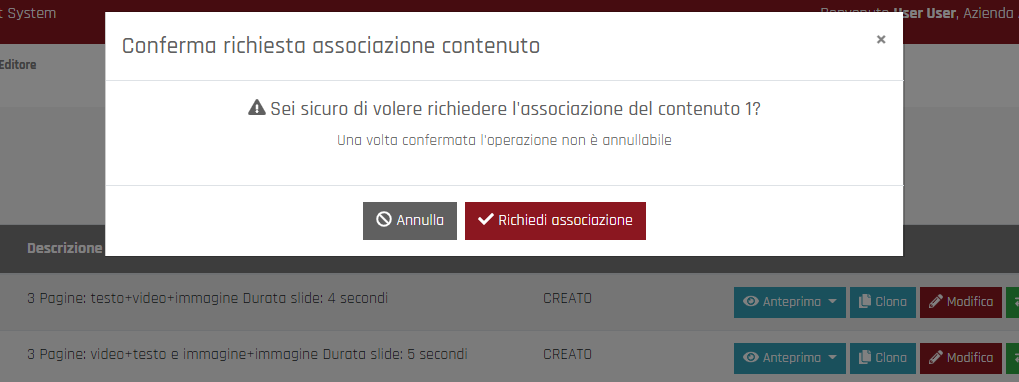
\includegraphics[width=1\textwidth]{associazione}
    \caption{Richiesta di associazione di un contenuto}
    \label{fig:figure28}
    \end{center}
\end{figure}

\subsection{Eliminazione di un contenuto}
Un contenuto potrebbe essere creato per errore o non più necessario, in questo caso può tornare utile l'eliminazione. L'eliminazione è irreversibile.
\begin{figure}[h]
    \begin{center}
    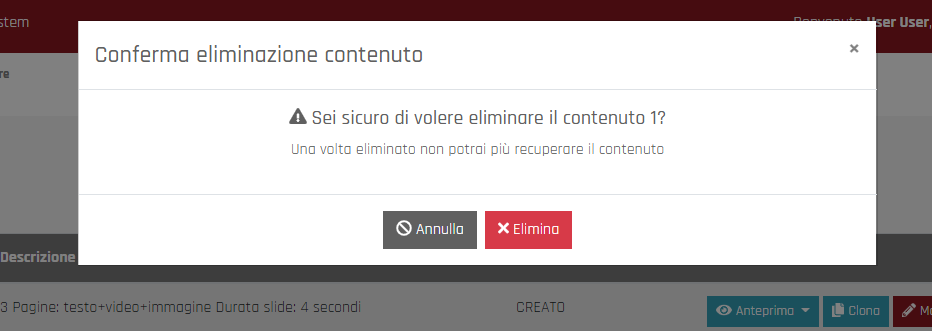
\includegraphics[width=1\textwidth]{eliminazione}
    \caption{Eliminazione di un contenuto}
    \label{fig:figure29}
    \end{center}
\end{figure}

\subsection{Audit}
La schermata di visualizzazione degli audit, raggiungibile dalla schermata principale, è visualizzabile da chiunque abbia effetuato il \textit{Login} e raccoglie varie informazioni sulle attività effettuate dagli utenti.
\begin{figure}[h]
    \begin{center}
    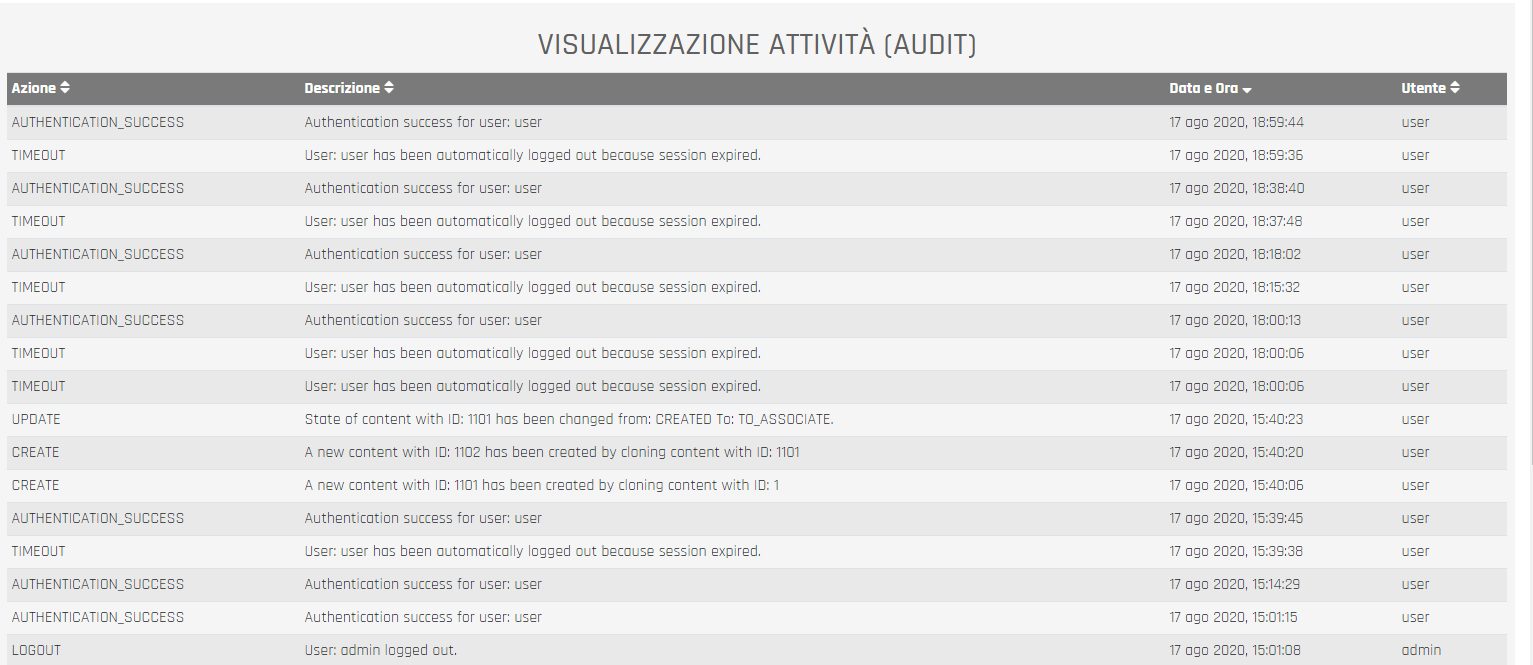
\includegraphics[width=1\textwidth]{audit}
    \caption{Visualizzazione audit}
    \label{fig:figure30}
    \end{center}
\end{figure}

%**************************************************************
\section{Documentazione}

%**************************************************************
\section{Test}
